


    %/////////////////////////////////////////////
	\section{Modèle analytique statique approché des lames flambées} 
    %/////////////////////////////////////////////
       	%*************
		\subsection{Établissement du modèle} 
		%*************		
	Nous avons précédemment simulé l'évolution du comportement statique d'une telle structure, en imposant des incréments de niveau de flambement. Il serait intéressant maintenant d'être capable de trouver la bonne géométrie pour les lames, en connaissant simplement le niveau énergétique injecté dans le bistable par l'oreille. Ce niveau résulte directement des paramètres $K$,$L$ et $x_0$ qui ont été définis précédemment. On aimerait alors lier ces trois paramètres à $K_{\varphi}$ et aux paramètres géométriques, ainsi que les paramètres matériau de d'une lame. Cette étape simplifierait le temps de dimensionnement des lames pour des niveaux d'entrée énergétiques différents.\\
%%%%%%%%%%%
\begin{figure}[!htbp]
\begin{center}
    \captionsetup{justification=centering}
	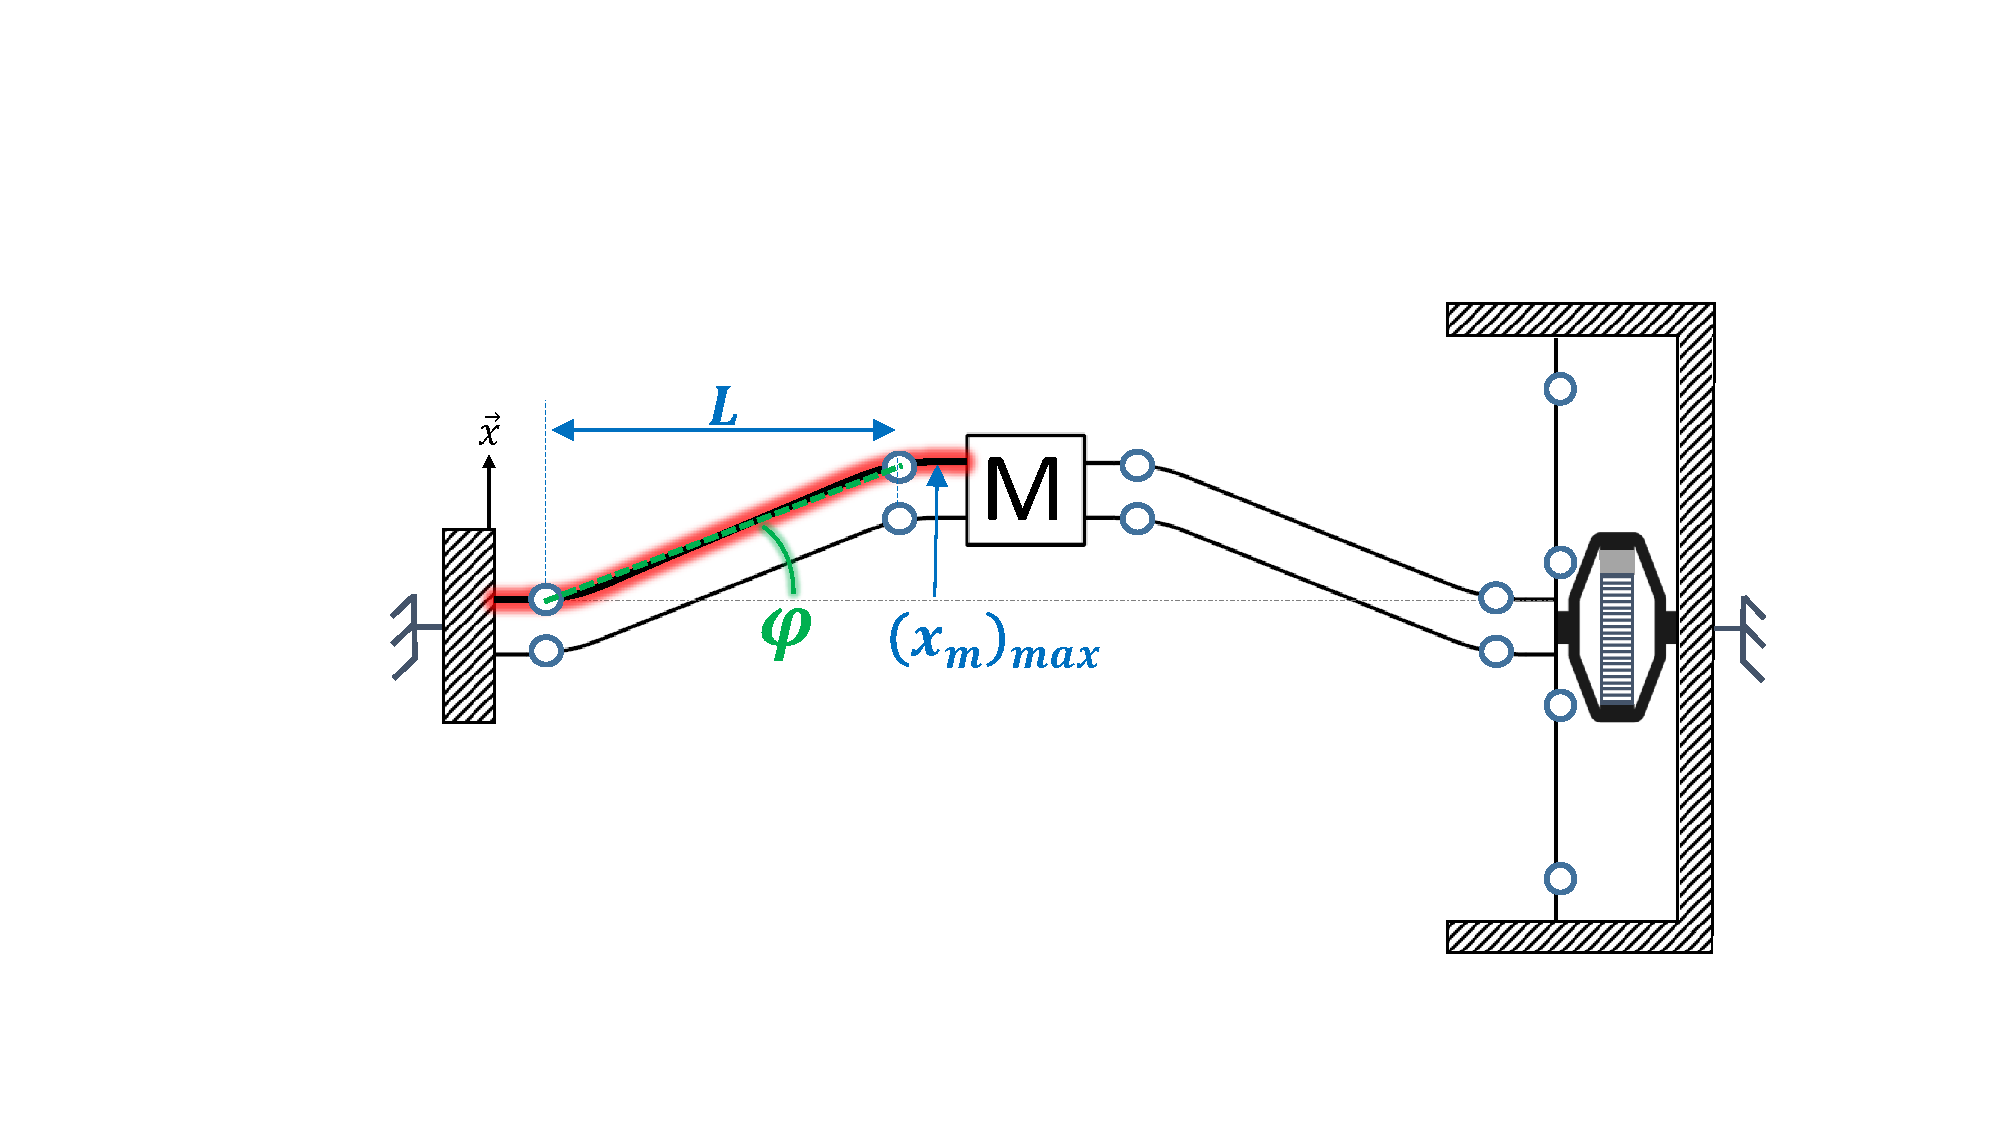
\includegraphics[trim={6cm 2.8cm 4cm 5cm},clip, width=0.7\textwidth]{../Chap4/Figure/OB_surbrillance_1_lame.pdf}
	\caption{L'OB à l'équilibre en $x_0$}
	\label{fig:OB_surbrillance_1_lame}
\end{center}
\end{figure}
%%%%%%%%%%%
Dans un souci de symétrie, le comportement mécanique de chacune des 4 lames est identique. Nous allons donc isoler le comportement d'une seule lame, mise en surbrillance sur la figure \ref{fig:OB_surbrillance_1_lame} pour établir un modèle analytique.
L'épaississement local aura pour rôle de rigidifier les pivots souples car la lame sera plus difficilement déformable sur cette portion. Cela dit il est important d'épaissir la lame localement, afin de minimiser l'impact des déformation résiduelles dues à la fabrication. L'idéal serait d'épaissir la lame de façon à minimiser l'impact sur la rigidité de la lame en flexion. C'est en effet possible si on arrive à épaissir la portion de la lame qui ne subit pas de déformation sous la sollicitation qui lui est demandée.
%%%%%%%%%%%%%%%%%%%%%
\begin{figure}[!htbp]
\begin{center}
    \captionsetup{justification=centering}
	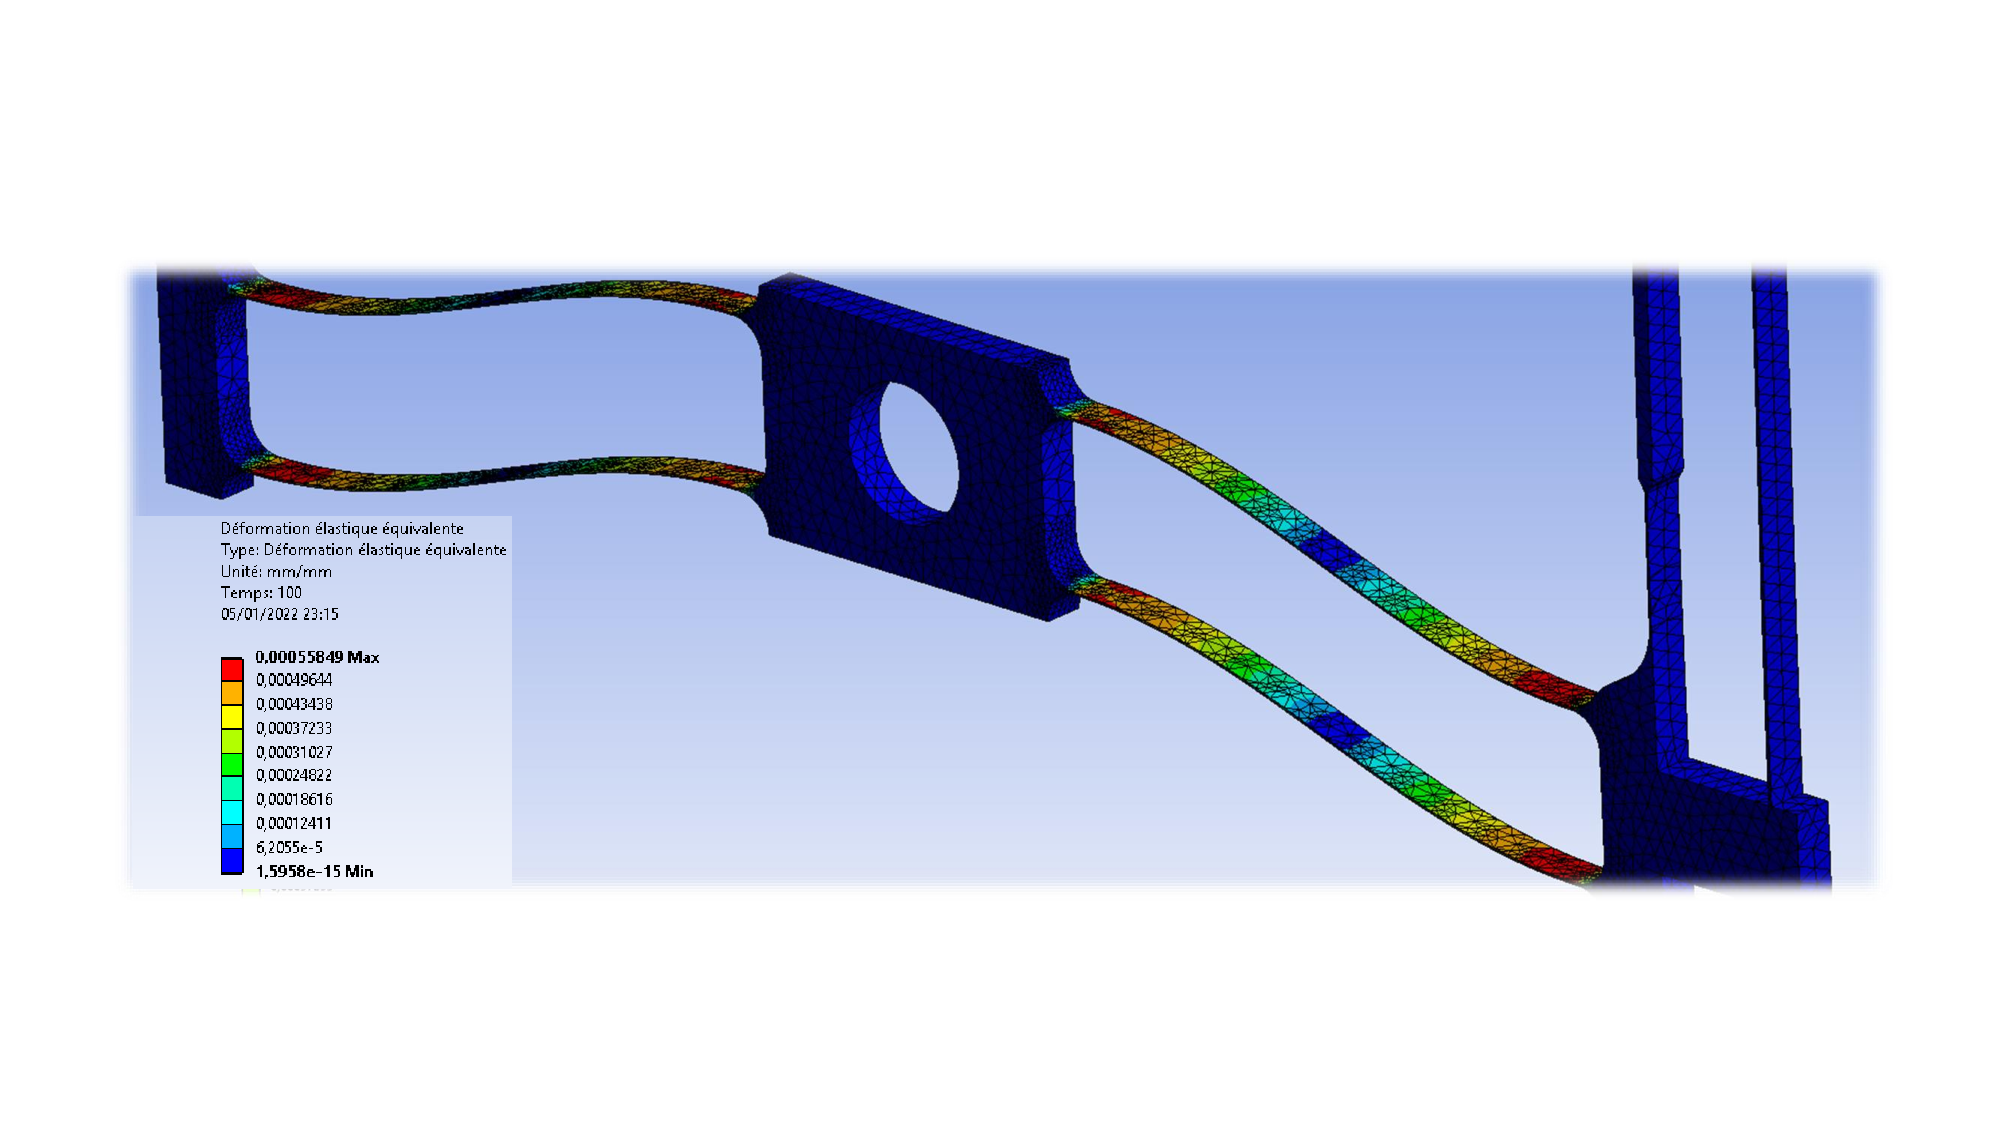
\includegraphics[trim={2cm 4cm 2cm 4cm},clip, width=\textwidth]{../Chap4/Figure/ANSYS_deformation.pdf}
	\caption{Déformation des lames horizontales sans épaississement}
	\label{fig:ANSYS_deformation}
\end{center}
\end{figure}
%%%%%%%%%%%
Sur la figure \ref{fig:ANSYS_deformation} on peut voir la déformation structurelle des lames horizontales sans épaississement, pour les mêmes conditions initiales et sollicitations externes que le modèle avec épaississements. On s'aperçoit alors que les déformations sont principalement concentrées aux extrémités des lames et sur un large portion au centre la lame subit des déformations 5 à 10 fois plus faibles. Le modèle analytique sera donc sous-dimensionné par rapport au modèle avec épaississements. Il suffira alors d'appliquer un coefficient de correction qui pourra être vérifié avec la méthode numérique développée précédemment.\\
	Sachant que le comportement des lames est linéaire sur toute la plage de fonctionnement, nous allons nous placer dans le cas extrême de $x_m = (x_m)_{max}$ et isoler une seule lame. Dans cette configuration, la lame peut être décomposée en deux lames symétriques encastrées-libres tel qu'on voit que la figure \ref{fig:OB_surbrillance_2_lames}. Leur longueur vaut alors $L/2$ et leur flèche à l'extrémité libre atteint pour chacune des lames :
\begin{equation}
		x_E =\frac{(x_E)_{max}}{2}
\label{eq:x_E=x_max/2}
\end{equation}
On introduit aussi la force normale $F_E$ qui induit cette flèche à l'équilibre statique, et depuis laquelle découlera la rigidité en flexion d'une demi-lame.\\
%%%%%%%%%%%
\begin{figure}[!htbp]
\begin{center}
    \captionsetup{justification=centering}
	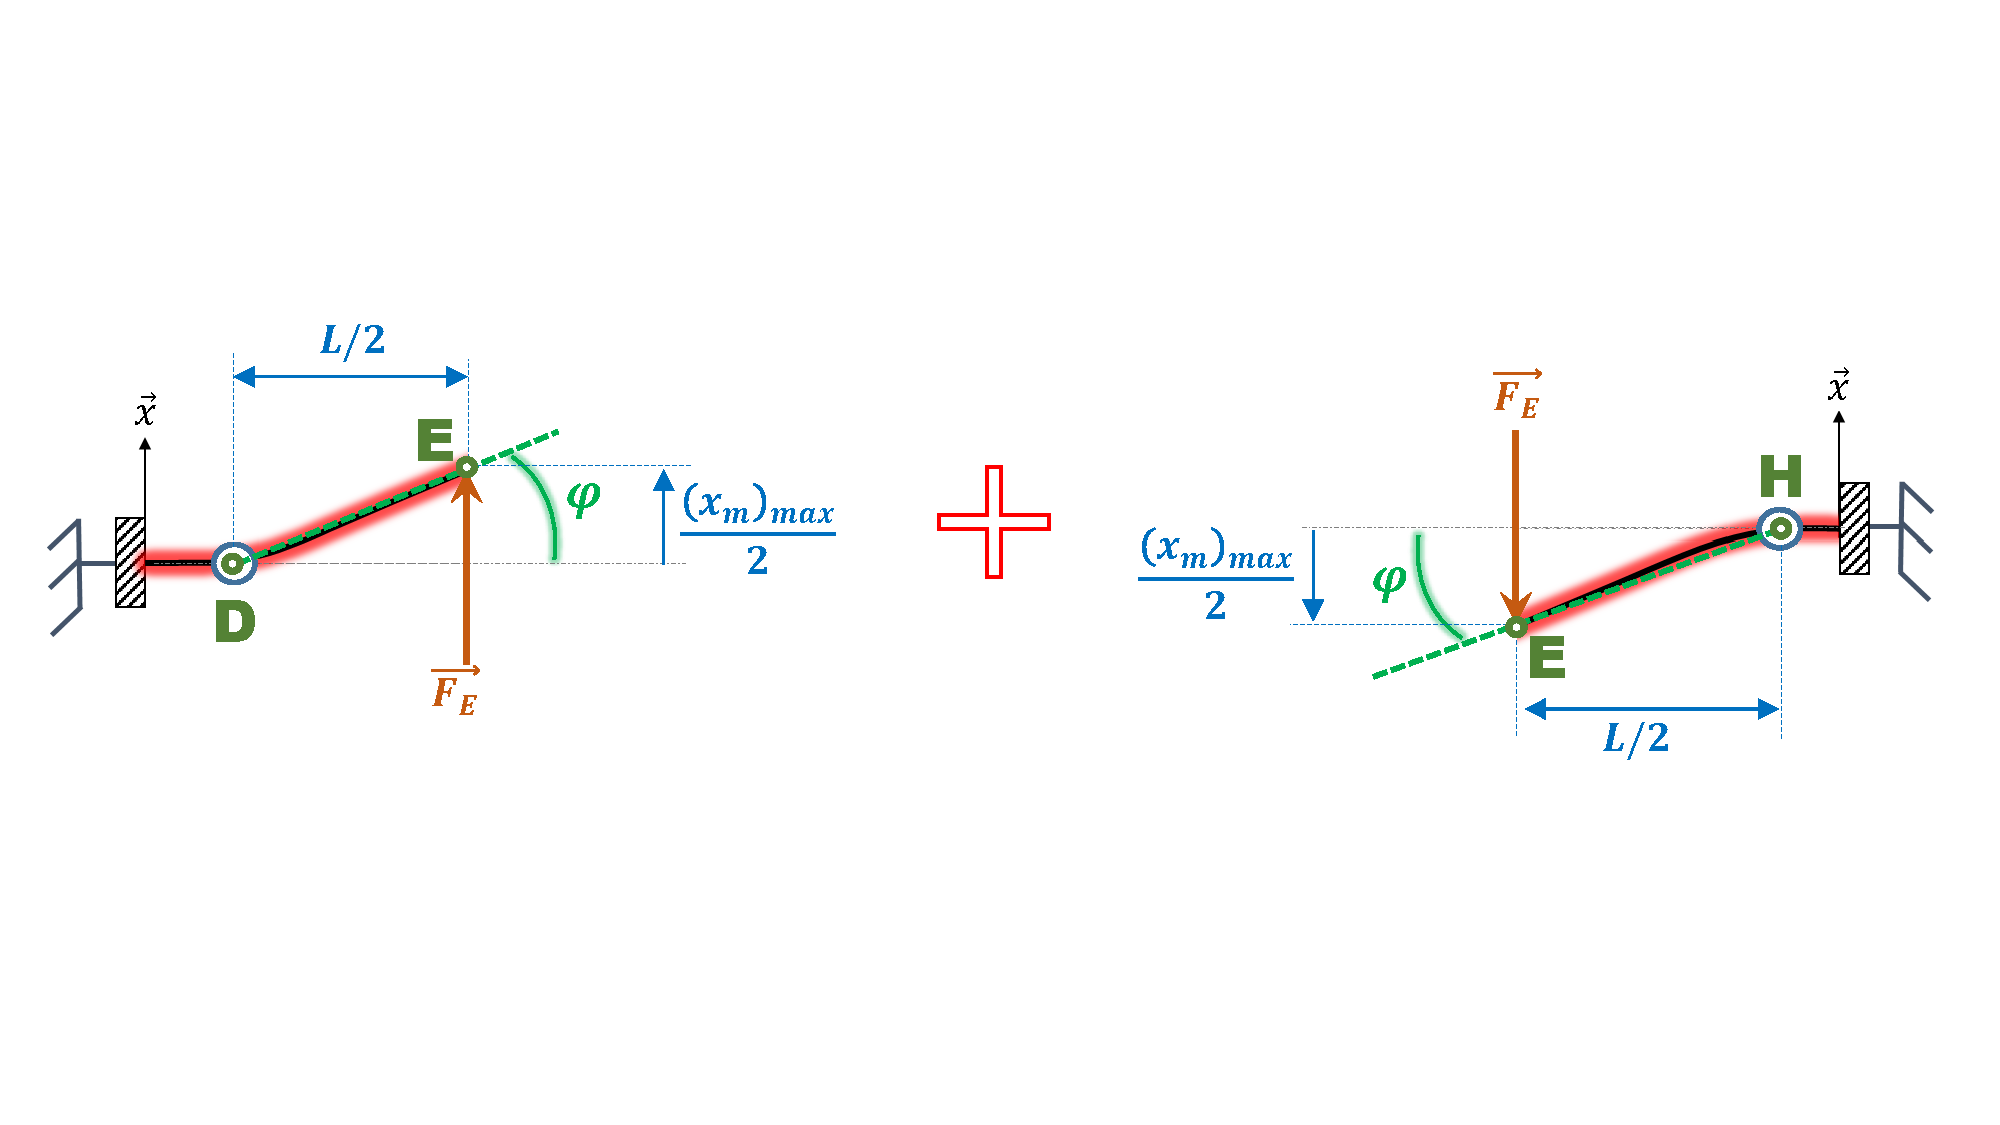
\includegraphics[trim={0cm 6cm 1cm 5cm},clip, width=\textwidth]{../Chap4/Figure/OB_surbrillance_2_lames.pdf}
	\caption{Hypothèse du comportement statique d'une lame de l'OB}
	\label{fig:OB_surbrillance_2_lames}
\end{center}
\end{figure}
%%%%%%%%%%%
Sur figure \ref{fig:poutre_flexion_simple} on montre le schéma de modélisation pour la demi-lame gauche. Naturellement le résultat sera similaire pour la demi lame droite par symétrie. On se positionne dans la théorie de déformation des poutres d'Euler-Bernoulli sans gauchissement pour la suite de l'étude analytique. 
%%%%%%%%%%%
\begin{figure}[!htbp]
\begin{center}
    \captionsetup{justification=centering}
	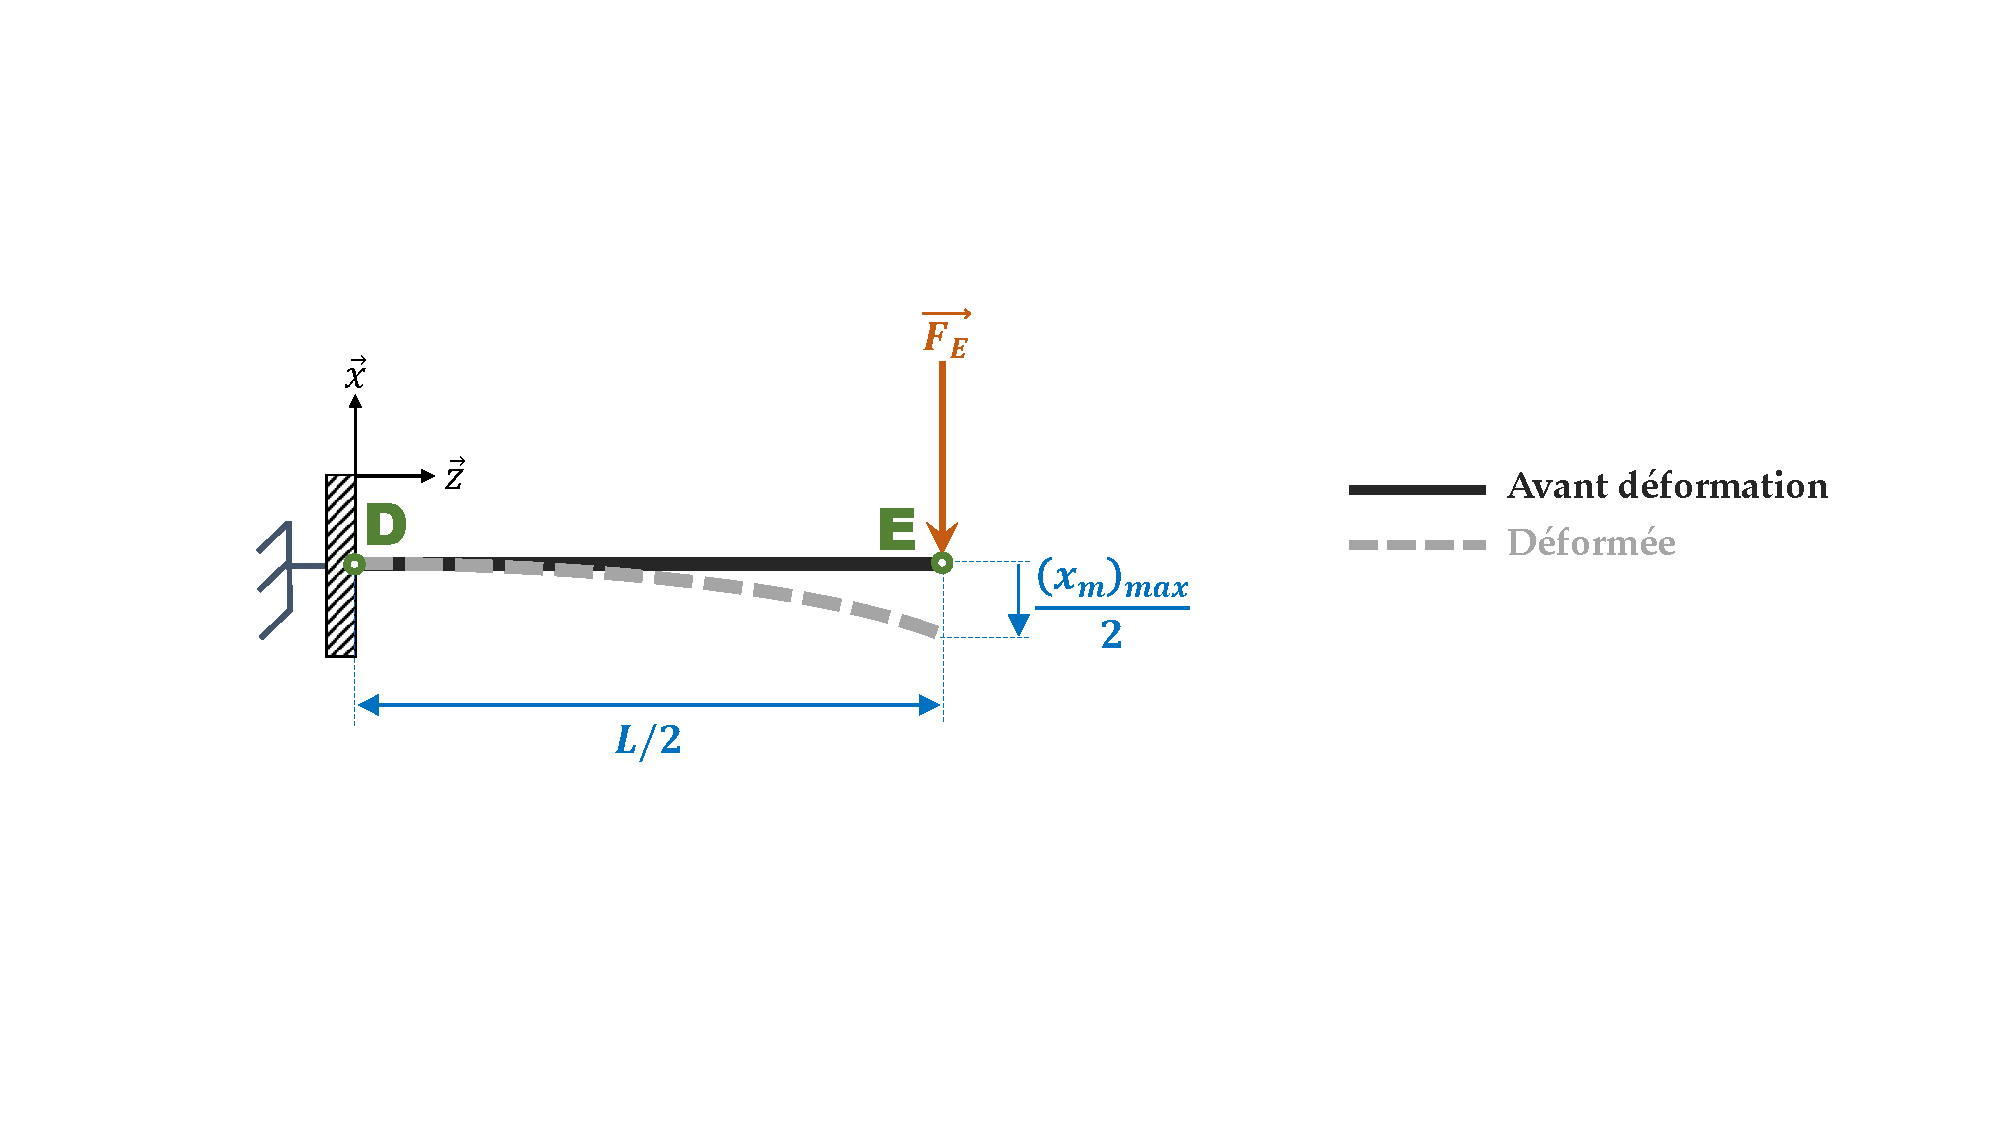
\includegraphics[trim={4cm 5.5cm 2.9cm 5cm},clip, width=\textwidth]{../Chap4/Figure/poutre_flexion_simple.pdf}
	\caption{Schéma poutre encastrée-libre en flexion simple}
	\label{fig:poutre_flexion_simple}
\end{center}
\end{figure}
%%%%%%%%%%%
L'équation de la déformée suivant de la lame suivant z peut alors être exprimée comme suit:
\begin{equation}
		x(z) = \frac{F_E}{6\ E\ I_h}\ z^2 \biggl( \frac{L}{2} - z \biggr)
\label{eq:deformée_encastrée-libre}
\end{equation} 
Où $I_h$ est le moment quadratique d'une lame horizontale. De cette équation on peut alors extraire la flèche maximale qui est à l'extrémité libre en $z=L/2$ :
\begin{equation}
		x_E = \frac{F_E\ (L/2)^3}{3\ E\ I_h}
\label{eq:fleche_encastrée-libre}
\end{equation} 	
De même, on peut exprimer la contrainte normale en flexion $\sigma _f$ grâce à l'équation :
\begin{equation}
	\sigma _f(z) = \frac{-F_E\ (L/2 - z)}{I_h}\ \biggl( \frac{e}{2} \biggr)
\end{equation}

D'autre part on peut exprimer la rigidité en rotation $K_{\varphi 2}$ d'une demi-lame qui est simplement le rapport du moment généré par l'angle de flexion :
\begin{equation}
		K_{\varphi 2} =  \frac{F_E\ (L/2)}{\arctan \biggl( \frac{(x_m)_{max}}{L} \biggr)}
\label{eq:K_phi demi-lame}
\end{equation}
$\varphi$ étant très faible on peut linéariser l'équation  \ref{eq:K_phi demi-lame} pour avoir :
\begin{equation}
		K_{\varphi 2} =  \frac{F_E\ L^2}{2\ (x_m)_{max}}
\label{eq:K_phi demi-lame linéarisée}
\end{equation}
En combinant alors les équations \ref{eq:x_E=x_max/2}, \ref{eq:K_phi_lim} et \ref{eq:K_phi demi-lame linéarisée} on peut exprimer la rigidité en rotation d'une demi-lame en fonction de ses paramètres géométriques et matériau comme suit :
\begin{equation}
		K_{\varphi 2} = \frac{6\ E\ I_h}{L}
		\label{eq:K_phi demi-lame final}
\end{equation}
Un lame complète est donc deux fois plus rigide, et donc :
\begin{equation}
		K_{\varphi} = \frac{12\ E\ I_h}{L}
		\label{eq:K_phi lame entière final}
\end{equation}